\documentclass[a4paper]{article}
\usepackage[utf8x]{inputenc}
\usepackage[T1]{fontenc}
\usepackage[MeX]{polski}
\usepackage{amssymb}
\usepackage{graphicx}
\usepackage{fancyhdr}
\usepackage{lastpage}
\usepackage{xcolor}
\usepackage{hyperref}
\definecolor{tableofcontents}{RGB}{0, 0, 0}
\hypersetup{
    colorlinks=true,
    urlcolor=blue,
    linkcolor=tableofcontents,
}

\pagestyle{fancy}
\fancyhf{}
\cfoot{ \thepage \hspace{1pt} / \pageref{LastPage}}
\lhead{Specyfikacja implementacyjna}
\rhead{\texttt{War Of Tanks}}


\begin{document}

\begin{titlepage}
    \begin{center}
        \vspace*{5cm}

            \Huge
            \textbf{Specyfikacja implementacyjna}

            \vspace{1cm}
            \Huge
            \texttt{War Of Tanks}

            \vspace{1.5cm}

            \large
            Aleksandra Michalska, Natalia Olszewska

            \vfill

            \vspace{3cm}

        \large 24.04.2021
    \end{center}
\end{titlepage}

\tableofcontents

\newpage

\section{Informacje og\'olne}

\subsection{Opis dokumentu}
\quad Dany dokument koresponduje ze \textit{Specyfikacj\k{a} funkcjonaln\k{a}}.

\subsection{\'Srodowisko implementacyjne}
\quad Projekt zostanie zaimplementowany w środowisku \textit{IntelliJ IDEA Community Edition 2021.1} oraz napisany w j\k{e}zyku \textit{Java 1.8}.

B\k{e}dzie przeznaczony do \'srodowisk Microsoft Windows, Linux (dystrybucje Mint oraz Ubuntu), Mac OS. 

W celu archiwizowania post\k{e}p\'ow pracy oraz sprawnego kontrolowania projektu zostanie wykorzystany system kontroli wersji: \textit{projektor.ee - system kontroli wersji Politechniki Warszawskiej}.

\subsection{Narz\k{e}dzia i programy towarzysz\k{a}ce tworzeniu}

\quad W czasie trwania projektu b\k{e}dzie konieczne skorzystanie z pomocy dodatkowych narz\k{e}dzi oraz program\'ow:

\begin{itemize}
    \item \textbf{projektor.ee} - system kontroli wersji,
    \item \textbf{LaTeX} - j\k{e}zyk pisania dokument\'ow projektu,
    \item \textbf{Overleaf} - platforma do sporz\k{a}dzania dokumentacji w j\k{e}zyku LateX,
    \item \textbf{IntelliJ IDEA Community Edition 2021.1} - \'srodowisko implementacyjne,
    \item \textbf{www.piskelapp.com} - strona internetowa do tworzenia grafiki pikselowej,
    \item \textbf{GIMP 2.10.20} - edytor graficzny,
    \item \textbf{ecrettmusic.com/play} - strona internetowa do generowania muzyki,
    \item \textbf{VLC media player} - odtwarzacz oraz konwerter multimedialny,
    \item \textbf{Swing} - biblioteka graficzna u\.zywana w j\k{e}zyku programowania Java,
    \item \textbf{Dysk Google} - dysk do przechowywania multimedi\'ow projektowych.
\end{itemize}


Wszelkie dodatkowe narz\k{e}dzia niewymienione powy\.zej zostan\k{a} dodane w dokumentacji uzupe\l{}niaj\k{a}cej po zako\'nczeniu implementacji projektu.

\subsection{Konwencja wprowadzania zmian w kontroli wersji}
\quad Wprowadzane zmiany w kodzie b\k{e}d\k{a} zatwierdzane zgodnie z konwencj\k{a} zaproponowan\k{a} na stronie \href{https://www.conventionalcommits.org/en/v1.0.0}{www.conventionalcommits.org}.

\subsection{Okre\'slenie kamieni milowych}

\quad W celu zobrazowania post\k{e}p\'ow faz projektu zosta\l{}a przyj\k{e}ta konwencja kamieni milowych jako tag\'ow w systemie kontroli wersji.

W momencie gdy implementacja fazy projektu zostanie zako\'nczona, w systemie kontroli wersji nale\.zy oznaczy\'c tag: \textit{MILESTONE\_COMPLETED\_NoXX},
gdzie \textit{XX} nale\.zy zamieni\'c na odpowiedni numer kamienia milowego (01, 02, 03, ..., 12).

Projekt b\k{e}dzie posiada\l{} dwana\'scie kamieni milowych: 

    
\begin{itemize}
    \item 01 - zako\'nczenie implementacji wygl\k{a}du okien \textit{StartFrame}, \textit{GameFrame}, \textit{SettingsFrame}, \textit{HelpFrame},
    \item 02 - skolekcjonowanie grafiki oraz \'scie\.zek d\'zwi\k{e}kowych dla projektu,
    \item 03 - opracowanie podstawowego poruszania si\k{e} czo\l{}g\'ow,
    \item 04 - zako\'nczenie implementacji \.zycia kom\'orek oraz kolonii,
    \item 05 - opracowanie struktury zachowania kom\'orki bomby,
    \item 06 - implementacja zarz\k{a}dzania kolizjami,
    \item 07 - opracowanie podstawowej struktury projektu,
    \item 08 - zako\'nczenie wst\k{e}pnej fazy testowania,
    \item 09 - zako\'nczenie nak\l{}adania poprawek,
    \item 10 - zako\'nczenie ostatecznej fazy testowania,
    \item 11 - zako\'nczenie refaktoryzacji kodu,
    \item 12 - zako\'nczenie obowi\k{a}zkowej cz\k{e}\'sci implementacji projektu.
    
\end{itemize}

\section{Opis klas i ich zależności}

\subsection{Diagram klas}

\quad W celu uproszczenia procesu implementacji zosta\l{} sporz\k{a}dzony diagram klas, jednak z przyczyn wizualnych jest on dost\k{e}pny pod danym
\href{https://drive.google.com/file/d/1yqUE8LddMVll-GYRUga39RELv98kOB-G/view?usp=sharing}{adresem}.

\subsection{Klasy}

\subsubsection{MainOfWar}
\quad \textbf{MainOfWar} b\k{e}dzie klas\k{a} pocz\k{a}tkow\k{a}. To w\l{}a\'snie w niej mo\.zna b\k{e}dzie znale\'z\'c metod\k{e} \textit{main}, odpowiedzialn\k{a} za uruchomienie programu. 
B\k{e}dzie posiada\'c jeden atrybut \textit{start} b\k{e}d\k{a}cym obiektem klasy \textbf{StartFrame}.

\subsubsection{StartFrame}

\quad Klasa, kt\'orej zadaniem b\k{e}dzie wy\'swietlenie podstawowego menu otrzyma mo\.zliwo\'s\'c uruchomienia ustawie\'n d\'zwi\k{e}ku, pokazania pomocy, za\l{}\k{a}czenia pliku konfiguracyjnego lub reset ustawie\'n otrzymanych z poprzednich plik\'ow konfiguracyjnych. 
Pojawi si\k{e} r\'ownie\.z opcja uruchomenia samej gry.

Klasa b\k{e}dzie dziedziczy\'c po \textbf{JFrame}, a wszelkie jej ustawienia b\k{e}d\k{a} mo\.zliwe do uruchomienia poprzez klikni\k{e}cie w odpowiedni przycisk – obiekty typu \textbf{JButton}.

Do atrybut\'ow tej klasy b\k{e}d\k{a} nale\.ze\'c obiekty typu \textbf{HelpFrame}, \textbf{GameFrame}, \textbf{SettingsFrame}, klasa posiada\'c b\k{e}dzie r\'ownie\.z obiekt przechowuj\k{a}cy ustawienia konfiguracyjne typu \textbf{ConfObject}. Dodatkowo, co zosta\l{}o wspomniane powy\.zej, menu zostanie zaimplementowane w postaci obiekt\'ow typu \textbf{JButton}.

Metody podziel\k{a} si\k{e} na \textit{manageButtons()}, odpowiedzialn\k{a} za kontrol\k{e} klikni\k{e}\'c menu, oraz \textit{readFile()}, kt\'ora b\k{e}dzie nadpisywa\l{}a i uaktualnia\l{}a obiekt przechowuj\k{a}cy ustawienia konfiguracyjne.

\subsubsection{HelpFrame}

\quad Klasa b\k{e}dzie mia\l{}a za zadanie wy\'swietli\'c podstawow\k{a} instrukcj\k{e} rozgrywki oraz obs\l{}ugi gry. B\k{e}dzie dziedziczy\'c po \textbf{JFrame}.

Atrybutem tej klasy najprawdopodobniej stanie si\k{e} pole tekstowe \textit{help} typu \textbf{JTextField} zawieraj\k{a}ce wszelkie potrzebne informacje dla graczy.

\subsubsection{ConfObject}

\quad Klasa \textbf{ConfObject} b\k{e}dzie mia\l{}a za zadanie przechowywa\'c wszelkie parametry potrzebne do skonfigurowania pojedynczej rozgrywki. Ka\.zdy jej atrybut otrzyma okre\'slone warto\'sci domy\'slne opisane w \textit{Specyfikacji funkcjonalnej}.

Atrybuty tej klasy b\k{e}d\k{a} typu \textbf{Integer}. 

Do jej metod wlicz\k{a} si\k{e} funkcje \textit{get} oraz \textit{set} dla ka\.zdego atrybutu. Dodatkowo zostanie zaimplementowana funkcja \textit{setPrimitiveParameters()} okre\'slaj\k{a}ca domy\'slne parametry, kt\'ora b\k{e}dzie prywatna – dost\k{e}pna tylko dla konstruktora tej klasy.

\subsubsection{GameFrame}

\quad Klasa \textbf{GameFrame} b\k{e}dzie tzw. \textit{sercem rozgrywki}. To w\l{}a\'snie ona skontroluje przebieg ca\l{}ej gry. Sama klasa b\k{e}dzie dziedziczy\'c po \textbf{JFrame}, dodatkowo b\k{e}dzie posiada\'c implementacje zdarze\'n kolizji, ruchu czo\l{}g\'ow, wystrzeliwania pocisk\'ow oraz struktury funkcjonowania kom\'orek i kolonii. Jej  konstruktor przyjmie argument typu \textbf{ConfObject} otrzymany od klasy \textbf{StartFrame}.

Do atrybut\'ow tej klasy zalicz\k{a} si\k{e}:
\begin{itemize}
    \item prawy czo\l{}g - typu \textbf{TankRight},
    \item lewy czo\l{}g - typu \textbf{TankLeft},
    \item panele punktacji - typu \textbf{JPanel},
    \item panele informacji o pociskach - typu \textbf{JPanel},
    \item panel czasu gry - typu \textbf{JPanel},
    \item bomba - typu \textbf{Bomb},
    \item lista spadaj\k{a}cych kom\'orek - typu \textbf{List<Cell>},
    \item lista kolonii r\'o\.znej liczby kom\'orek - typ\'ow \textbf{List<Colony2>}, 
    
    \textbf{List<Colony3>}, \textbf{List<Colony4>}, \textbf{List<Colony5>},
    \item lista pocisk\'ow lewego czo\l{}gu - typu \textbf{List<BulletL>},
    \item lista pocisk\'ow prawego czo\l{}gu - typu \textbf{List<BulletR>},
    \item obiekt konfiguracyjny - typu \textbf{ConfObject},
    \item czasomierz - typu \textbf{Timer}.
\end{itemize}

Do metod b\k{e}d\k{a} si\k{e} zalicza\'c:

\begin{itemize}
    \item konstruktor - przyjmuj\k{a}cy argument typu \textbf{ConfObject},
    \item \textit{manageKeyboard} - obs\l{}uguj\k{a}cy wej\'scie klawiatury,
    \item \textit{addPoints()} - dodaj\k{a}cy punktacj\k{e} do odpowiedniego panelu w momencie zdobycia punkt\'ow przez kt\'orego\'s z graczy, przyjmuje argumenty \textit{points} oraz \textit{which} typu \textbf{Integer}. 
    \item \textit{manageColisionOnLeft()} - sprawdzaj\k{a}cy kolizje pocisk\'ow lewego czo\l{}gu,
    \item \textit{manageColisionOnRight()} - sprawdzaj\k{a}cy kolizje pocisk\'ow prawego czo\l{}gu,
    \item \textit{setPanels()} - okre\'slaj\k{a}cy wygl\k{a}d paneli,
    \item \textit{setObstacle()} - okre\'slaj\k{a}cy podstawowe ustawienia kolonii oraz kom\'orek,
    \item \textit{setBullet()} - przygotowuj\k{a}cy odpowiedni\k{a} struktur\k{e} pocisk\'ow dla czo\l{}g\'ow,
    \item \textit{setConf()} - ustawiaj\k{a}cy obiekt konfiguracyjny zgodnie z tym przekazanym przez konstruktor, przyjmuje argument typu \textbf{ConfObject},
    \item \textit{saveScreenShoot()} - zapisuj\k{a}cy obraz po zako\'nczeniu rozgrywki do pliku o rozszerzeniu graficznym.
\end{itemize}

\subsubsection{SettingsFrame}

\quad Klasa b\k{e}dzie dziedziczy\'c po \textbf{JFrame}. Stanie si\k{e} odpowiedzialna za zmiany ustawie\'n g\l{}o\'sno\'sci \'scie\.zek d\'zwi\k{e}kowych. Do mo\.zliwych opcji b\k{e}d\k{a} dost\k{e}pne: 
\begin{itemize}
    \item \'sciszenie,
    \item  podg\l{}o\'snienie,
    \item wy\l{}\k{a}czenie,
    \item w\l{}\k{a}czenie.
\end{itemize}
Ka\.zda z tych opcji b\k{e}dzie dost\k{e}pna w postaci przycisk\'ow przy ka\.zdej kategorii d\'zwi\k{e}kowej:
\begin{itemize}
    \item muzyka startowa,
    \item d\'zwi\k{e}k wystrza\l{}u pocisk\'ow,
    \item muzyka w czasie rozgrywki.
\end{itemize}

Do atrybut\'ow tej klasy zostan\k{a} przydzielone:
\begin{itemize}
    \item przyciski - typu \textbf{JButton},
    \item warto\'s\'c g\l{}o\'sno\'sci muzyki startowej - \textit{volumeOfMusicStart},
    \item warto\'s\'c g\l{}o\'sno\'sci muzyki podczas gry - \textit{volumeOfMusicPlaying},
    \item warto\'s\'c g\l{}o\'sno\'sci muzyki wystrza\l{}u pocisku - \textit{volumeOfBullets}.
\end{itemize}

Do metod nale\.ze\'c b\k{e}d\k{a}: 
\begin{itemize}
    \item \textit{turnOnMusic()} - w\l{}\k{a}czaj\k{a}ca muzyk\k{e},
    \item \textit{turnOffMusic()} - wy\l{}\k{a}czaj\k{a}ca muzyk\k{e},
    \item \textit{volumeUp()} - podg\l{}o\'sniaj\k{a}ca muzyk\k{e},
    \item \textit{volumeDown()} - \'sciszaj\k{a}ca muzyk\k{e},
    \item \textit{getVolumeOfMusicStart()} - zwracaj\k{a}ca warto\'s\'c g\l{}o\'sno\'sci muzyki startowej,
    \item \textit{getVolumeOfBullets()} - zwracaj\k{a}ca warto\'s\'c g\l{}o\'sno\'sci wystrza\l{}u pocisk\'ow,
    \item \textit{getVolumeOfMusicPlaying()} - zwracaj\k{a}ca warto\'sci g\l{}o\'sno\'sci muzyki podczas rozgrywki,
    \item \textit{setButtons()} - ustawiaj\k{a}ca podstawowy wygl\k{a}d przycisk\'ow,
    \item \textit{manageButtons()} - kontroluj\k{a}ca operacje na przyciskach.
    
\end{itemize}

\subsubsection{Colony}

\quad Klasa \textbf{Colony} b\k{e}dzie klas\k{a} abstrakcyjn\k{a}, s\l{}u\.z\k{a}c\k{a} do implementacji klas \textbf{Colony2}, \textbf{Colony3}, \textbf{Colony4}, \textbf{Colony5}.
Klasa ta b\k{e}dzie odpowiedzialna za funkcjonowanie struktury kolonii z\l{}o\.zonej z pewnej (od 2 do 5) liczby kom\'orek. 

Do atrybut\'ow tej klasy abstrakcyjnej nale\.ze\'c b\k{e}d\k{a}:
\begin{itemize}
    \item liczba kom\'orek, z jakiej sk\l{}ada si\k{e} kolonia - typu \textbf{Integer},
    \item lista kom\'orek - typu \textbf{List<Cell>},
    \item liczba punkt\'ow mo\.zliwa do uzyskania po likwidacji kolonii - typu \textbf{Integer},
    \item pr\k{e}dko\'s\'c poruszania si\k{e} kolonii - typu \textbf{Integer}.
\end{itemize}

Do metod klasy nale\.ze\'c b\k{e}d\k{a}:
\begin{itemize}
    \item \textit{setPrimaryParameters()} - ustawiaj\k{a}ca pocz\k{a}tkowe warto\'sci kolonii,
    \item \textit{getPoints()} - zwracaj\k{a}ca liczb\k{e} mo\.zliwych punkt\'ow,
    \item \textit{getVelocity()} - zwracaj\k{a}ca warto\'s\'c pr\k{e}dko\'sci kolonii,
    \item \textit{getHowMany()} - zwracaj\k{a}ca liczb\k{e} wszystkich kom\'orek w kolonii,
    \item \textit{isDead()} - zwracaj\k{a}ca warto\'s\'c typu \textbf{Boolean} czy kolonia zosta\l{}a zlikwidowana,
    \item \textit{setPoints()} - zmieniaj\k{a}ca warto\'s\'c punkt\'ow mo\.zliwych do uzyskania, przyjmuje argument typu \textbf{Integer},
    \item \textit{setVelocity()} - zmieniaj\k{a}ca warto\'s\'c pr\k{e}dko\'sci kolonii, przyjmuje argument typu \textbf{Integer},
\end{itemize}

\subsubsection{Cell}

\quad     Klasa b\k{e}dzie mia\l{}a za zadanie kontrolowa\'c struktur\k{e} pojedynczej kom\'orki.

Do jej atrybut\'ow b\k{e}d\k{a} nale\.ze\'c:

\begin{itemize}
    \item lista kolor\'ow jakie przyjmowa\'c b\k{e}dzie kom\'orka zale\.znie od liczby \.zy\'c - typu \textbf{List<Color>},
    \item liczba \.zy\'c kom\'orki - typu \textbf{Integer},
    \item rozmiar boku kom\'orki - typu \textbf{Integer},
    \item pr\k{e}dko\'s\'c kom\'orki - typu \textbf{Integer},
    \item liczba punkt\'ow za likwidacj\k{e} kom\'orki - typu \textbf{Integer}. 
\end{itemize}

W sk\l{}ad metod b\k{e}d\k{a} wchodzi\'c funkcje \textit{set} do zmiany parametr\'ow kom\'orki oraz \textit{get} do otrzymywania odpowiednich warto\'sci atrybut\'ow. 
Dodatkowo klasa b\k{e}dzie posiada\'c metody:
\begin{itemize}
    \item \textit{getShoot()} - wywo\l{}ywan\k{a} przy kolizji z pociskiem,
    \item \textit{setPrimaryCellParameters()} - ustawiaj\k{a}c\k{a} podstawowe warto\'sci dla kom\'orki,
    \item \textit{isDead()} - sprawdzaj\k{a}c\k{a} czy kom\'orka zosta\l{}a zlikwidowana, zwraca warto\'s\'c typu \textbf{Boolean}.
\end{itemize}

\subsubsection{Bomb}

\quad Klasa b\k{e}dzie odpowiada\l{}a za struktur\k{e} kom\'orki bomby.

B\k{e}dzie posiada\'c dwa atrybuty. Jeden okre\'slaj\k{a}cy czy zosta\l{}a uderzona, a drugi przechowuj\k{a}cy grafik\k{e} samej bomby.

Do metod tej klasy b\k{e}d\k{a} si\k{e} wlicza\'c: pobranie i ustawienie warto\'sci atrybutu czy zosta\l{}a uderzona oraz ustawienie wst\k{e}pnych warto\'sci kom\'orki bomby.

\subsubsection{Bullet}

\quad Klasa abstrakcyjna s\l{}u\.z\k{a}ca p\'o\'zniejszej implementacji obiekt\'ow \textbf{BulletR} oraz \textbf{BulletL}, b\k{e}dzie posiada\'c atrybuty okre\'slaj\k{a}ce promie\'n i pr\k{e}dko\'s\'c pocisku.

Dodatkowo do jej metod b\k{e}d\k{a} si\k{e} zalicza\'c \textit{get} oraz \textit{set} dla ka\.zdego z atrybut\'ow.


\subsubsection{TankLeft oraz TankRight}

\quad Klasy bli\'zniacze b\k{e}d\k{a} implementowa\l{}y struktury odpowiednio czo\l{}gu lewego oraz prawego. 

W atrybutach znajd\k{a} si\k{e} panele odpowiadaj\k{a}ce korpusom czo\l{}g\'ow oraz lufom, pozycja czo\l{}g\'ow na osi x oraz k\k{a}t pod jakim b\k{e}dzie si\k{e} aktualnie znajdowa\'c lufa.

W metodach zostan\k{a} zaimplementowane opcje poruszania czo\l{}giem oraz luf\k{a}, a tak\.ze mo\.zliwo\'sci uzyskania warto\'sci atrybut\'ow pozycji i k\k{a}ta (\textit{getPosition()}, \textit{getAngle}).

\subsubsection{BodyL oraz BodyR}

\quad Klasy bli\'zniacze dziedzicz\k{a}ce po \textbf{JPanel}. B\k{e}d\k{a} odpowiada\l{}y za struktur\k{e} korpusu czo\l{}gu, a dok\l{}adniej zmian\k{e} odpowiedniej grafiki. 

W atrybutach b\k{e}d\k{a} si\k{e} znajdowa\'c dwie grafiki korpusu. Ich zmiana w momencie poruszenia czo\l{}giem b\k{e}dzie symulowa\'c ruch.

Do metod b\k{e}d\k{a} nale\.ze\'c:
\begin{itemize}
    \item \textit{changeBody()} - zmieniaj\k{a}ca grafik\k{e} korpusu,
    \item \textit{setBody()} - ustawiaj\k{a}ca podstawowe parametry korpusu.
\end{itemize}


\subsubsection{BarrelL oraz BarrelR}

\quad Bli\'zniacze klasy b\k{e}d\k{a} odpowiada\l{}y za struktury luf. B\k{e}d\k{a} dziedziczy\'c po \textbf{JPanel}.

Poniewa\.z lufa b\k{e}dzie posiada\'c wiele grafik odpowiadaj\k{a}cych k\k{a}tom, zostan\k{a} one umieszczone w li\'scie \textbf{List<Image>}.

Klasa b\k{e}dzie posiada\'c trzy metody:
\begin{itemize}
    \item \textit{changeBarrelUp()} - zmieniaj\k{a}ca grafik\k{e} lufy o k\k{a}t w g\'or\k{e},
    \item \textit{changeBarrelDown()} - zmieniaj\k{a}ca grafik\k{e} lufy o k\k{a}t w d\'o\l{},
    \item \textit{setBarrels()} - ustawiaj\k{a}ca podstawowe parametry panelu lufy.
\end{itemize}

\subsection{Zale\.zno\'sci mi\k{e}dzy klasami}

\quad W projekcie mamy na celu wykorzystanie trzech rodzaj\'ow relacji: agregacji (kompozycji), dziedziczenia, asocjacji. 
Du\.zy nacisk zostanie na\l{}o\.zony na niski poziom dziedziczenia oraz na jak najwi\k{e}ksz\k{a} modularno\'s\'c. 

\subsection{Wzorce projektowe}

\quad W p\'o\'zniejszych etapach projektu mo\.ze zaistnie\'c potrzeba wykorzystania pewnych wzorc\'ow projektowych, np. fabryki abstrakcji (dla implementacji czo\l{}g\'ow). 

\section{Multimedia}

\subsection{Grafika}

\quad Wszelkie grafiki zosta\l{}y lub zostan\k{a} wykonane na stronie \textit{www.piskelapp.com}, a nast\k{e}pnie dopracowane w \textit{GIMP} (patrz  \textit{Rysunek \ref{fig:piskel}}).

 \begin{figure}[h]
                \centering
                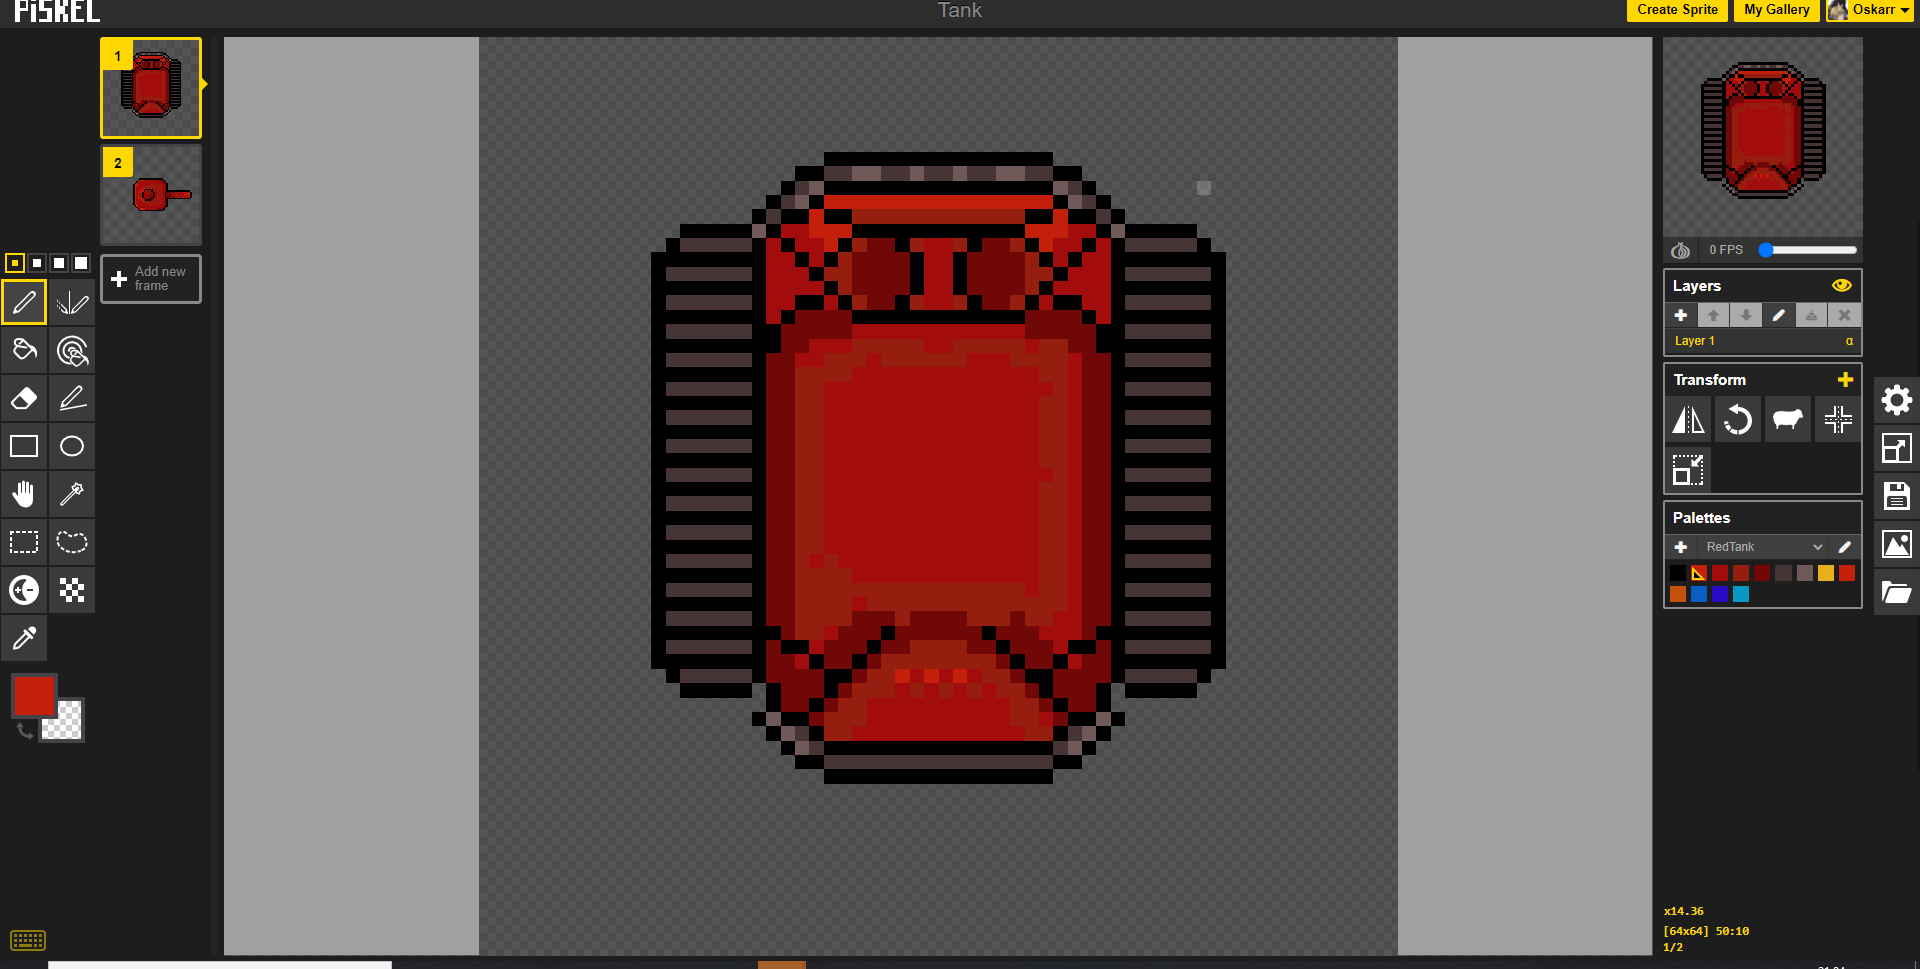
\includegraphics[scale=0.23]{Piskel.png}
		\caption{Proces wytwarzania grafiki}
		\label{fig:piskel}
\end{figure}

\subsection{Muzyka}

\quad \'Scie\.zki d\'zwi\k{e}kowe zostan\k{a} wygenerowane i dopracowane na stronie \textit{ecrettmusic.com}.
B\k{e}d\k{a} one edytowane w \textit{VLC media player}.

\section{Testowanie}
\subsection{Wygl\k{a}d test\'ow}

\quad Testowanie zostanie zaimplementowane w trakcie tworzenia pojedynczych klas oraz w fazach testowania. Kod b\k{e}dzie przetestowany za pomoc\k{a} automatycznych test\'ow jednostkowych (JUnit).

\subsection{Najwa\.zniejsze elementy do przetestowania}

\quad W testach nacisk zostanie na\l{}o\.zony na przetestowanie wszelkich wyj\k{a}tk\'ow dotycz\k{a}cych przekazywanych oraz zapisywanych parametr\'ow.


\subsection{Opis test\'ow kluczowych}

\begin{enumerate}
    \item Dodawanie punkt\'ow za zabicie kom\'orki przez odpowiedni czo\l{}g.
    \item Odpowiednia liczba wystrzelonych pocisk\'ow.
    \item Poprawna obs\l{}uga odczytu pliku konfiguracyjnego.
    \item Poprawna obs\l{}uga zmiany parametr\'ow po czasie.
    \item Prawid\l{}owy zapis obrazu okna po zako\'nczeniu gry.
    \item Obs\l{}uga wej\'scia klawiatury.
    \item Prawid\l{}owa obs\l{}uga zabiegu hermetyzacji atrybut\'ow oraz metod klas.
    \item Poprawna obs\l{}uga zmian ustawie\'n d\'zwi\k{e}ku.
\end{enumerate}
    




\end{document}

